\section{Evaluation}

\subsection{Experimental setup}



\subsection{Experimental setup}


\subsection{Consideration of delaying event}

\begin{figure} [htb]
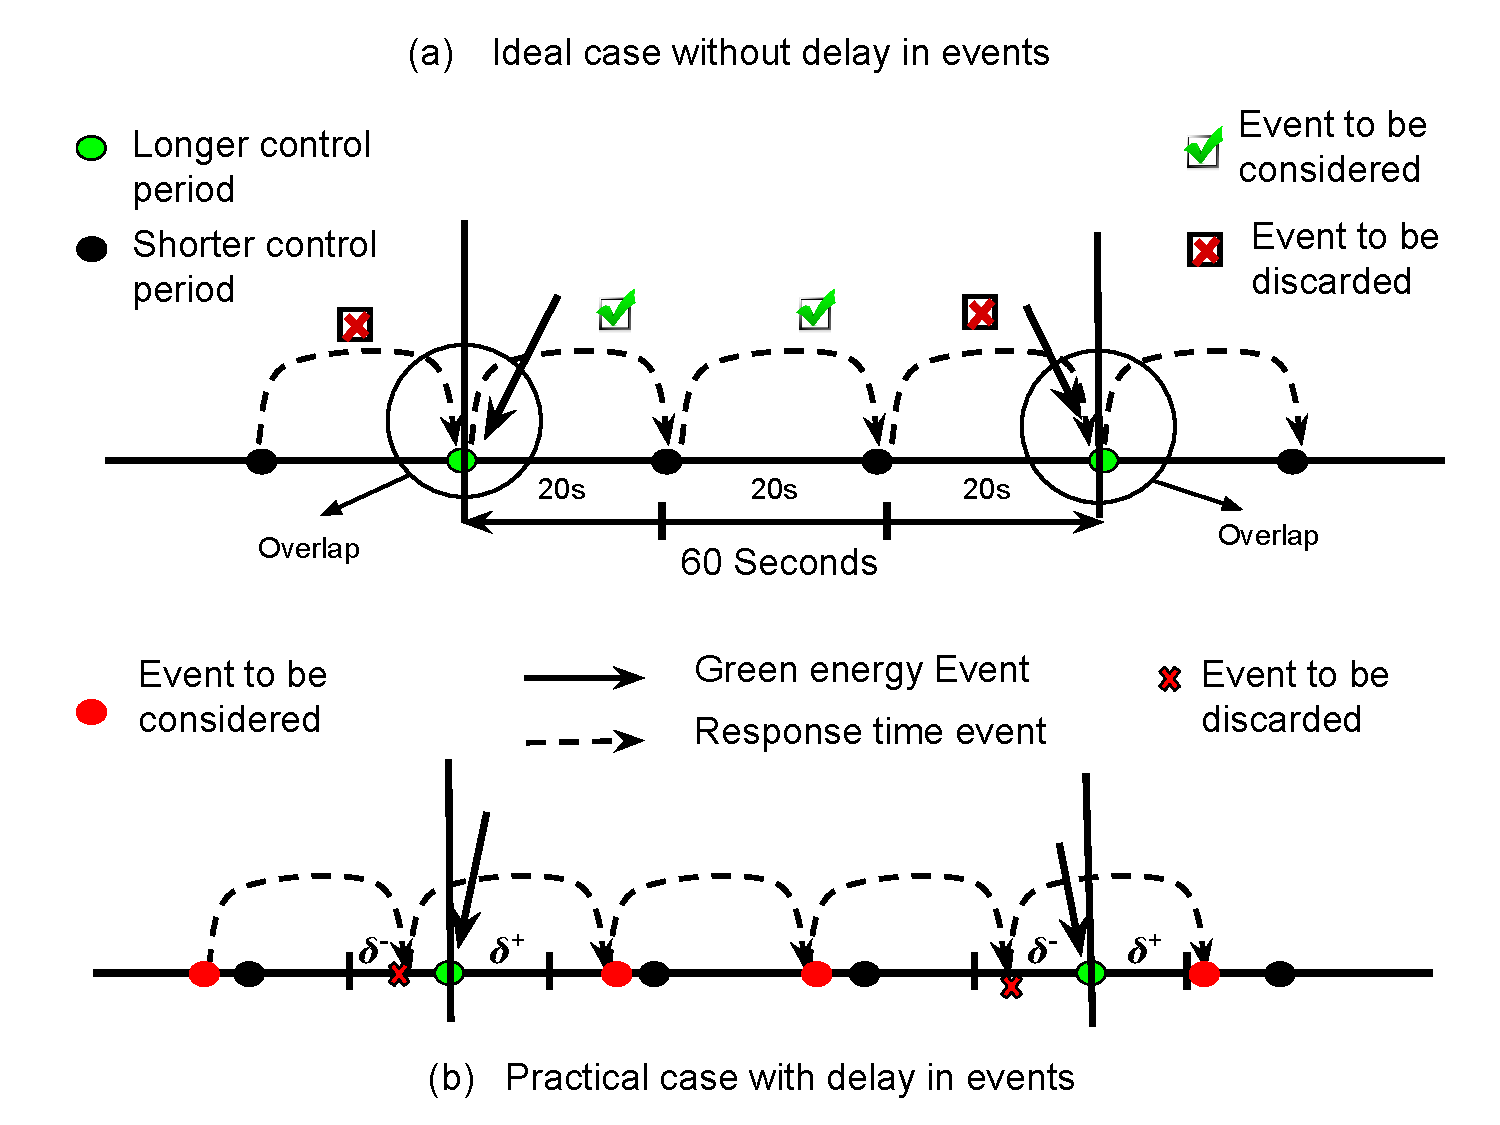
\includegraphics[scale=.35]{Graphs/implementation_UCC.pdf}
\caption{Algorithm implementation in detail}
\label{fig:implementation} 
\end{figure}

From Section \ref{saas-controller}, we see that, \emph{GE-C} controller has inner and outer loops which are activated in different time-scales and push events to the controller to make decision. In our experiments, outer (longer control period) and inner (shorter control period) loops are activated in each 60 seconds and 20 seconds respectively, which is showed in Figure \ref{fig:implementation}. Ideally, if both kind of events arrive without any delay, two different events will overlap each other. As our motivation is to maximize of green energy usage for \emph{GE-C} controller, we always make primary decision based on the green energy event pushed by IaaS by ignoring the response time event which is activated as inner loop, if both the event arrives concurrently. Concretely, it suggests that, between two big decision events in 60 seconds, we consider only two inner loop events and take actions if it is necessary indicated in Figure \ref{fig:implementation}(a).

But in case of delaying of any event, the scenario will not follow Figure \ref{fig:implementation}(a). As discussed before, the primary decision always depends on green energy event. Even though we receive response time event, no action is taken unless the system's response is high. Therefore, in case of delaying of response time event by micro to milliseconds, effects to the system remain almost unchangeable. In contrast, if the event delays by couple of seconds, for instance, inner loop event arrives just before or after the primary decision is made, it might affect the system dynamics to achieve the goal. To tackle the problem, we define a safety distance, denoted by $\delta^t$ to ensure that the controller does not take any action if response time event arrives in between "\textit{PrimaryDecision - $\delta^t$}" and "\textit{PrimaryDecision + $\delta^t$}". Figure \ref{fig:implementation}(b) illustrates the phenomena by an example. For our case, we choose safety distance as, $\delta^t$ = Time frequency of inner loop / $2$, which is equal to 10 seconds in our experiments.



\subsection{Results}
\paragraph{Response time}
\paragraph{Energy Consumption}
\paragraph{Cost analysis}


